In questa sezione viene illustrato lo sviluppo dei dataset, che contengono le osservazioni che verranno utilizzate dagli algoritmi di machine learning nel prossimo capitolo (\ref{4.0}). \vspace{7pt} \\
Dopo aver recuperato la lista di metadati, sono state estratte le features destinate ai dataframe, i quali condividono gli stessi domini presentati nel Paragrafo \ref{3.1.1}. Sono stati realizzati due insiemi di dati per distinguere le informazioni in base ai modelli di classificazione impiegati, attuando a seconda delle circostanze una previa fase di preprocessing. \vspace{7pt} \\
Nel caso di modelli di linguaggio naturale, che si formalizzano sulla comprensione e interpretazione di informazioni testuali, è stato preferito mantenere le risorse nel loro formato originale. Viceversa, per gli algoritmi che richiedono rappresentazioni vettoriali delle variabili in ingresso, sono state adeguate delle operazioni di pre-elaborazione, mirate a migliorare la qualità dei dati e a garantire una maggiore efficacia durante l'etichettatura.
\begin{lstlisting}[language=python, caption=Creazione del primo dataset]
import pandas

data = {
    "DOI": [metadata.DOI for metadata in list_metadata],
    "Title": [metadata.title for metadata in list_metadata],
    "Keywords": [metadata.keyword for metadata in list_metadata],
    "Abstract": [metadata.abstract for metadata in list_metadata],
    "Introduction": [metadata.intro for metadata in list_metadata]
}

df_not_cleaned = pandas.DataFrame(data=data).dropna(
    subset=["DOI", "Title", "Abstract"]
)
df_not_cleaned.head()
\end{lstlisting}
\begin{figure}[h]
    \centering
    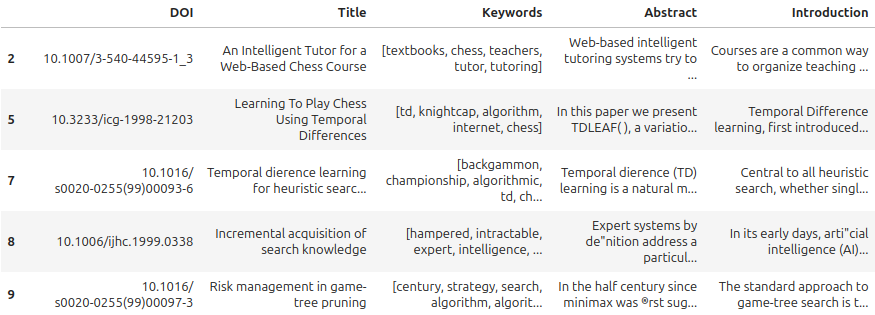
\includegraphics[width=1.0\textwidth]{img/img5.png}
    \caption{Raffigurazione del primo dataset}
    \label{fig:3.3-3.2}
\end{figure}
Al termine della computazione, il dataset ha generato una matrice di dimensione:
\begin{center}
    $N\times d = 1131 \times 5$
\end{center}
dove $N$ è il numero di righe, mentre $d$ rappresenta la cardinalità delle colonne. Questo insieme di dati è utilizzato esclusivamente per modelli di linguaggio naturale. \\
Per il secondo dataset è stata implementata la stessa logica di sviluppo, ma applicando una funzione dedicata alla pre-elaborazione della risorsa data in input. Il preprocessing effettuato sui testi, appartenenti agli articoli scientifici dell'archivio, è sintetizzabile nei seguenti passaggi:
\begin{itemize}
    \renewcommand{\labelitemi}{-}
    \item \textbf{Traduzione in inglese}. \\
    Dopo una breve analisi, sono emersi alcuni documenti della raccolta scritti in lingue differenti. Per tale ragione, affinché sia garantita un'omogeneità dei dati, sono stati tradotti in inglese.
    \item \textbf{Conversione del testo in minuscolo}. \\
    Il testo è convertito in minuscolo, evitando in questo modo casi in cui sia stabilita l'importanza di una parola in base alla sua forma.
    \item \textbf{Tokenizzazione}. \\
    L'informazione testuale è suddivisa nella lista di parole che la compone, rimuovendo articoli, congiunzioni e \textbf{stopwords}. Per la suddivisione in ciascuna parola, è stato impiegato un \textbf{tokenizer} implementato mediante la libreria \textbf{RegexTokenizer}.
    \item \textbf{Lemmatizzazione}. \\
    Ciascuna parola individuata nello step precedente, viene convertita nella sua forma originale, ignorando coniugazione verbali e convertendo i sostantivi al singolare.
\end{itemize}
\begin{lstlisting}[language=python, caption=Preprocessing delle informazioni testuali]
from langdetect import detect
from nltk.stem import WordNetLemmatizer
from nltk.tokenize import RegexpTokenizer
from deep_translator import GoogleTranslator

lemmatizer = WordNetLemmatizer()
tokenizer = RegexpTokenizer(r"[a-zA-Z]+")

def preprocess_field(field: str) -> List[str]:
    try:
        if detect(field) != "en":
            field = GoogleTranslator(source="auto", target="en").translate(field)

        text = field.lower()
        tokens = tokenizer.tokenize(text)

        tokens = [token for token in tokens if len(token) > 2]
        tokens = [token for token in tokens if token not in set_stopwords]

        return [lemmatizer.lemmatize(token) for token in tokens]
    except Exception:
        return [" "]
\end{lstlisting}
\begin{figure}[H]
    \centering
    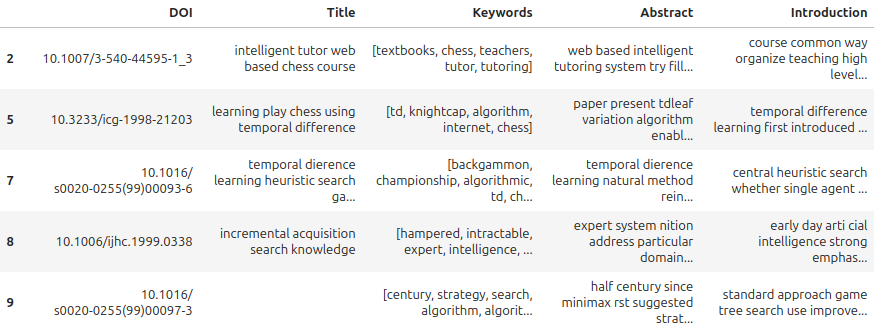
\includegraphics[width=1.0\textwidth]{img/img6.png}
    \caption{Raffigurazione del secondo dataset}
    \label{fig:3.3-3.3}
\end{figure}
Il dataframe circoscritto possiede la stessa dimensione del dataset precedente, a differenza del fatto che le istanze raccolte al suo interno sono successive alle operazioni di pre-elaborazione citate.